\chapter[Trigger Hardware and Software]{Trigger Hardware and Software
\footnote{
  $CVS~revision~ $Id: trigger.tex,v 1.8 2003/12/17 03:59:48 gen Exp $ $
}
\footnote{Authors: R.Michaels \email{rom@jlab.org}}
}

\section{Overview}
\par
The Hall A trigger was designed by the
University of New Hampshire.
Here we give a brief overview of the 
hardware arrangement,
the logic of the trigger, and the usage
of the software control.
Diagrams of the hardware layout are shown in
accompanying figures.

\par

Scintillators make the main trigger 
in each spectrometer arm. For coincidence experiments a 
coincidence is formed between the spectrometer arms.   
The main trigger is formed by requiring that scintillator 
planes S1 and S2 both fired (and both phototubes of the 
paddles that got a hit) in a simple overlap. To repeat, 
the trigger requires that one paddle in S1 and one in 
S2 both got a hit in both of their PMTs (4 PMTs total).  
The coincidence between spectrometers is formed in an 
overlap AND circuit.  The Right Spectrometer singles 
triggers are called T1, the Left Spectrometer triggers 
are called T3, and the coincidence triggers are T5.   
Other triggers might be formed which require other detectors 
to measure the efficiency of the main trigger. The most 
important is T2 on R-arm and T4 on L-arm, whose definition 
has changed over time but typically require 2 out of 3 
from among the S1, S2, and \Cherenkov{} detectors (i.e. the 
"or" of S1 is used, etc).

The Hall A HRS trigger system is remotely configured by 
CAMAC modules.   The main change that can occur during 
an experiment is in the delays required to adjust the 
timings of triggers which change with momentum and 
particle ID relevant for coincidence setup only.   
Of course for single arm running one may just use the 
defaults, but it may still be a wise investment in 2 
minutes time to download in order to make sure of 
the state of the modules.   If the power is turned off, 
the CAMAC modules certainly must be reprogrammed. 
Instructions to download the trigger are given below.

The trigger design is quite flexible and it
is relatively easy to add detectors to define
new trigger types or to modify existing ones,
so long as the detector is fast enough.
The trigger supervisor also allows for the
possibility of 2nd level triggers which could
be used for a later decision.


\infolevone{

\section{Components}
The trigger schematics is shown in Fig. \ref{fig:strig} and \ref{fig:ctrig}.

\begin{figure}
\begin{center}
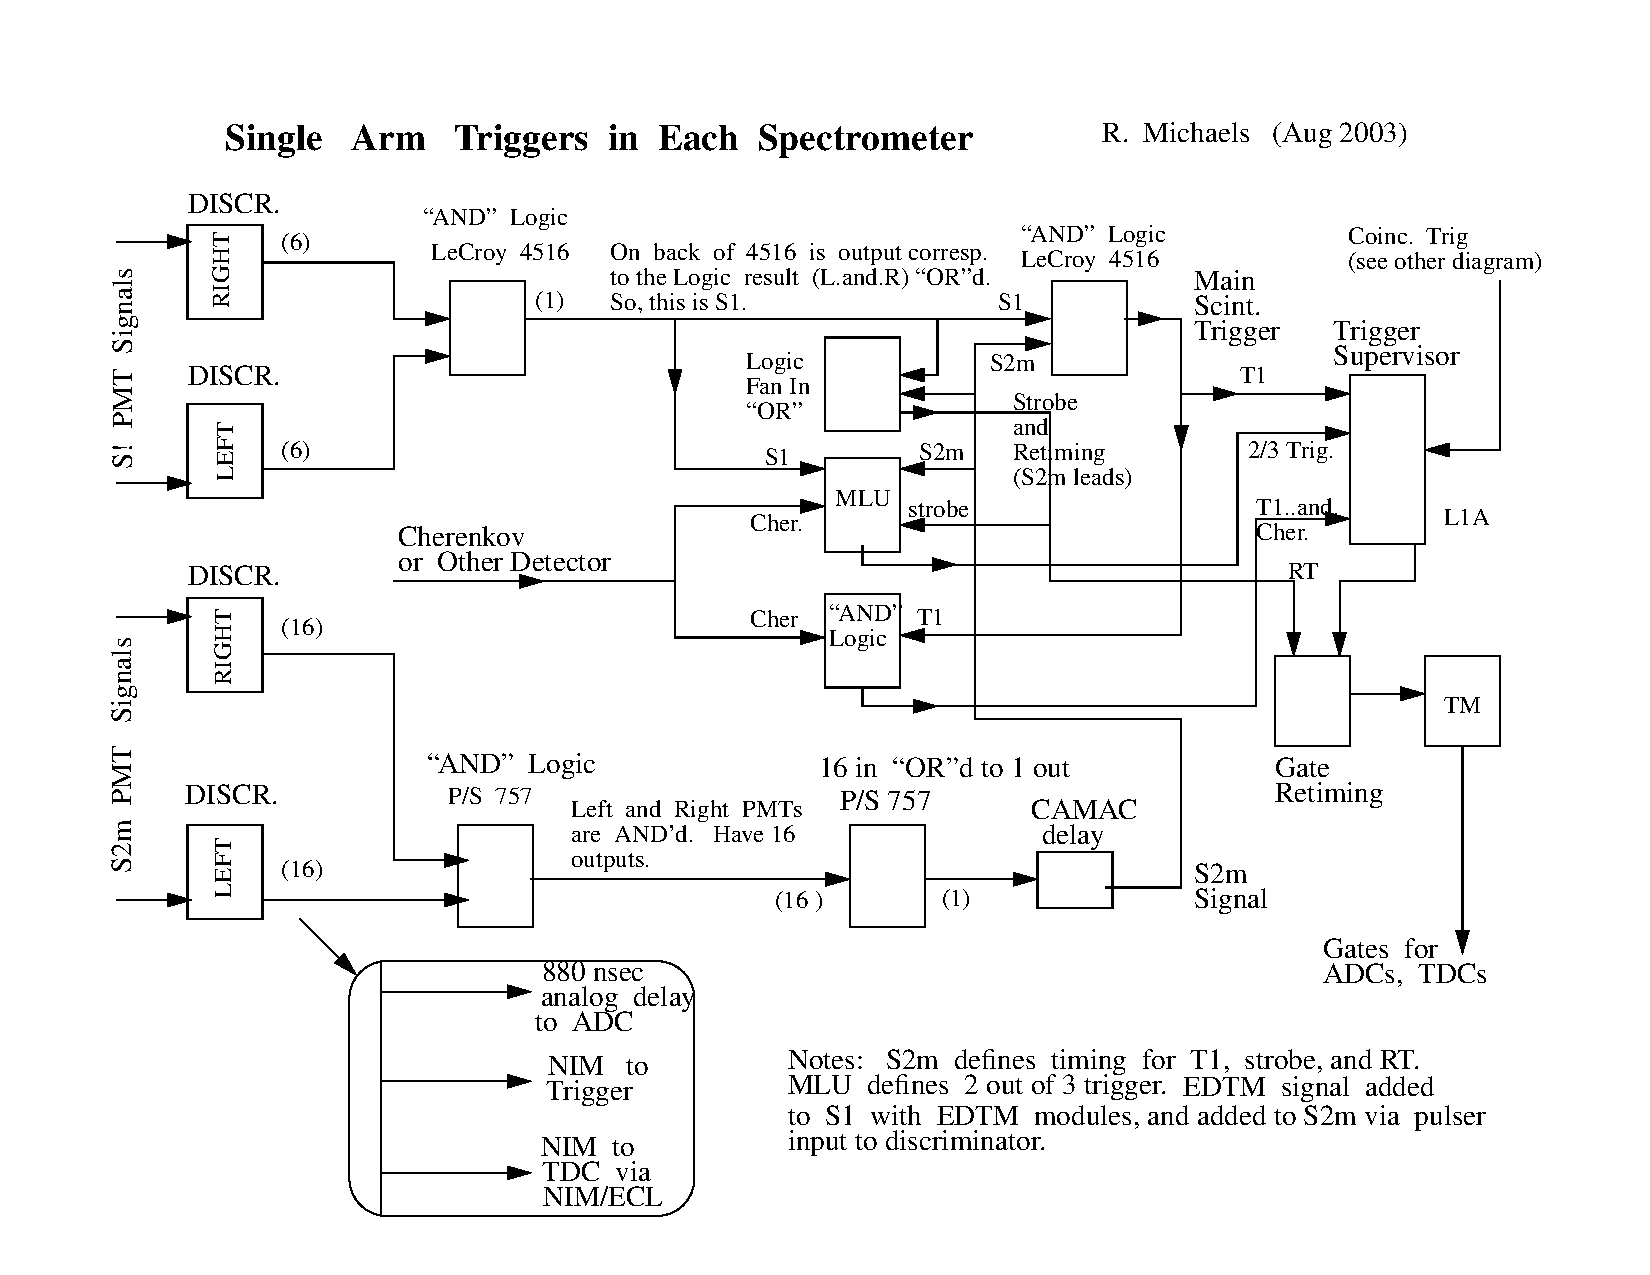
\includegraphics[angle=0,width=15cm,clip]{strig}
{\linespread{1.}
\caption[Data Acquisition: Single Arm Trigger]{Single Arm Trigger Circuit.}
\label{fig:strig}}
\end{center}
\end{figure}

\begin{figure}
\begin{center}
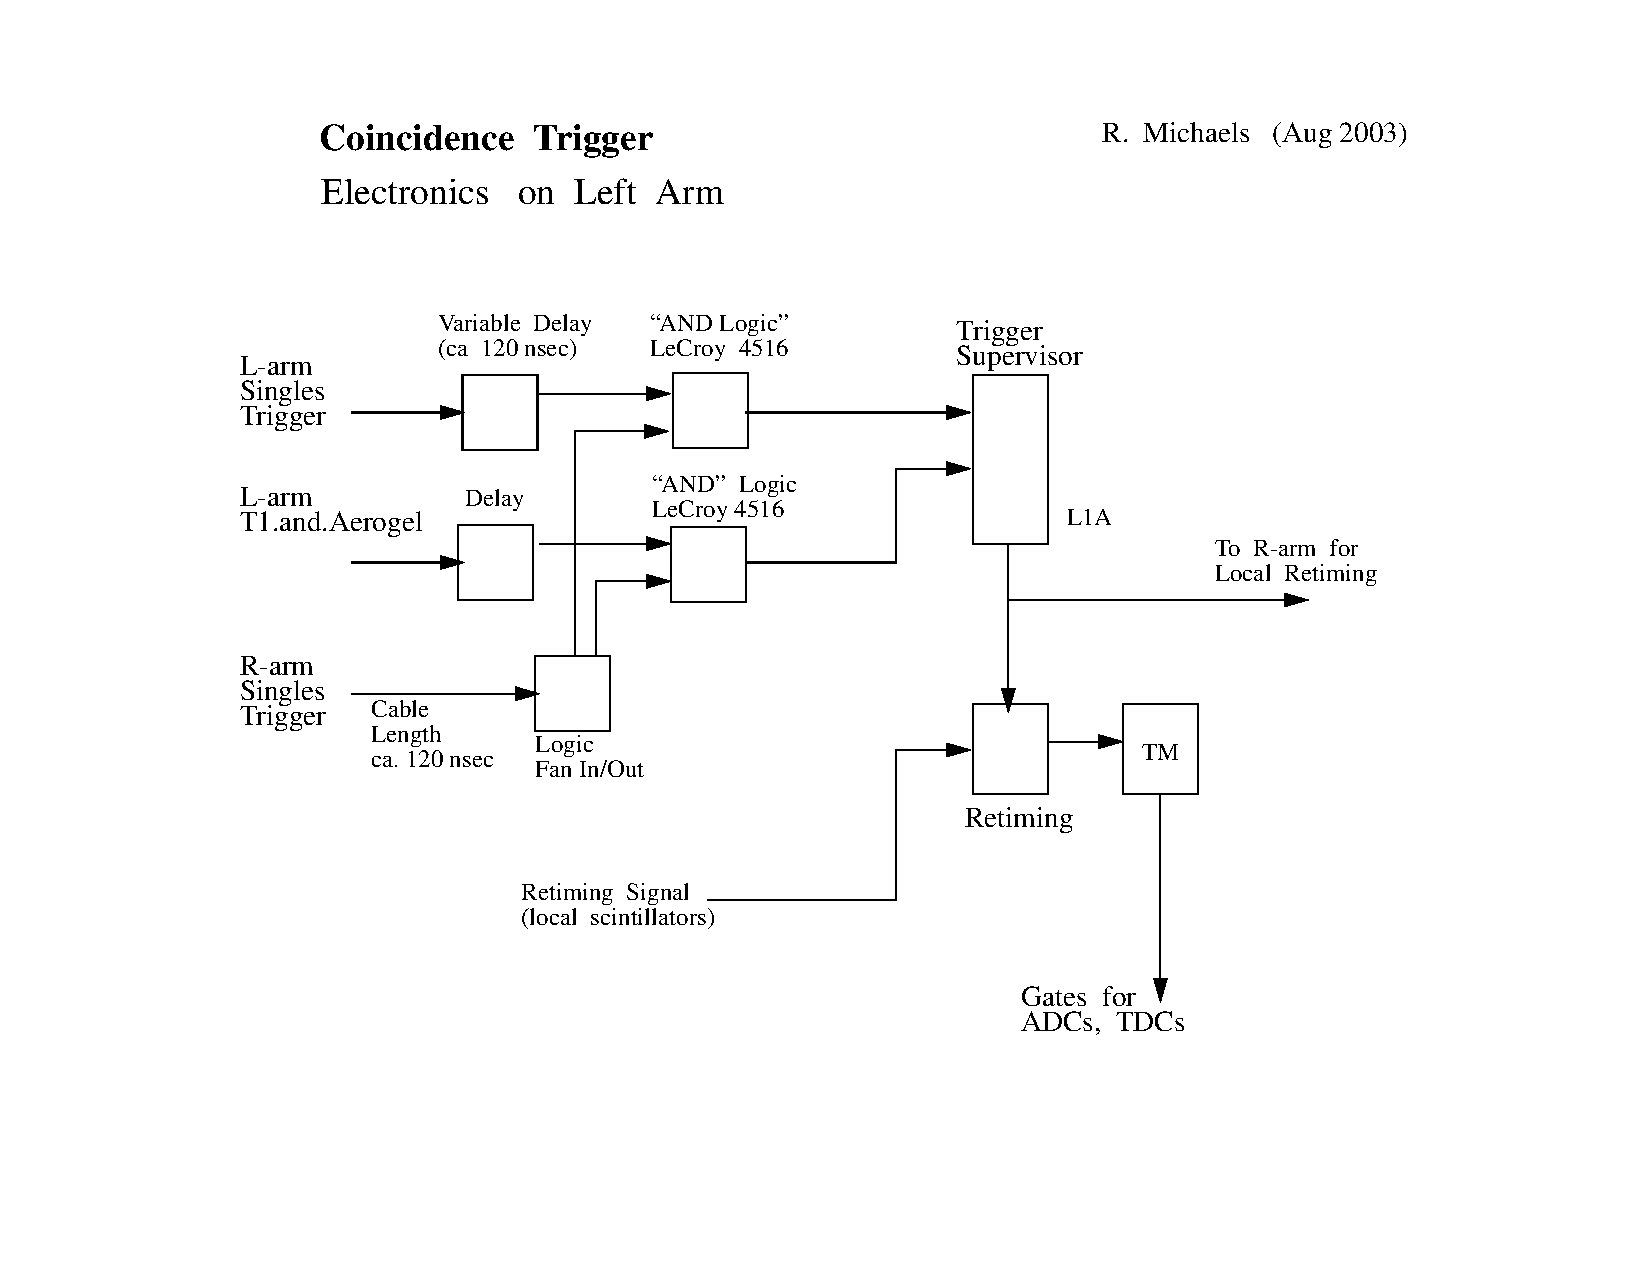
\includegraphics[angle=0,width=15cm,clip]{coinc_03}
{\linespread{1.}
\caption[Data Acquisition: Coincidence Trigger]{Coincidence Trigger Circuit.}
\label{fig:ctrig}}
\end{center}
\end{figure}
} %infolev

\infolevtwo{

\par
Here we describe the software control
of the CAMAC modules involved in the trigger.
The software control was written by 
Tim Smith and Jeff Vieregg of MIT with
some input from Bob Michaels.
There are four types of modules that
are controlled:
\begin{list}{\arabic{enumi}.~}{\usecounter{enumi}\setlength{\itemsep}{-0.15cm}}
  \item Discriminators; 
  \item Delay Units; 
  \item Memory Lookup Units; 
  \item AND/OR Modules.
\end{list}

Here are the instructions to download the trigger.
First login to the ADAQ Linux box \mycomp{adaql1} or \mycomp{adaql2} 
(and no others) as \mycomp{atrig} account.   (E.g. \mycomp{ssh adaql1 -l atrig}).   
The Run Coordinator should know the password.  
Type \mycomp{trigsetup}.   A self-explanatory graphical user 
interface pops up, where if you are in a coincidence 
experiment setup you must enter the momenta and particle 
ID's and then press "Download" and WAIT for it to finish 
and do not press \mycomp{Ctrl-C}.   However, for single arm 
running like Spin Duality or GDH, just press "Download" 
with the defaults, and WAIT for it to finish and do 
not press \mycomp{Ctrl-C}.   The user should look for suspicious 
error messages in the window from which trigsetup was 
launched, e.g. to check if connection to the crate is ok. 

\par
If individual modules need to be modified
for test purposes etc. (e.g. to change thresholds),
one may use the expert mode.
Login to an ADAQ linux box as explained above, 
then type \mycomp{trigsetup mapfile} where mapfile is 
the name of the trigger map file.   Some examples 
of map files are in \mycomp{/home/atrig/trigger}, see 
\mycomp{trigger\_left.map} and \mycomp{trigger\_right.map} for the 
left and right spectrometers respectively.     
These are default databases.   One can modify 
each module on the fly, save the database, etc.   

\par

After you download, a record of what was sent is put into a file \\ 
\mycomp{/home/atrig/trigger/trigger.setup} 
which gets put automatically into the electronics 
logbook ``halog''.   Also, whenever a CODA run is 
started, this file is inserted as a special event 
type 136 at the start of run.   This will be the 
setup IF the download was successful.   It is also 
interesting to know what is actually in CAMAC, but 
that can only be done in expert mode, and the delays
cannot be read from CAMAC.
The simplest way to be sure about what is in the 
trigger is to download again. 

} % infolev


\begin{safetyen}{10}{15}
\subsection{Authorized  Personnel} 
\end{safetyen}
The authorized personnel is shown in table \ref{tab:trig:personnel}.
\begin{namestab}{tab:trig:personnel}{Trigger: authorized personnel}{%
      Trigger: authorized personnel.}
  \RobertMichaels{\em Contact}
  \BodoReitz{}
\end{namestab}

% $Header: /group/halla/analysis/cvs/tex/osp/src/daq_trig/trigger.tex,v 1.8 2003/12/17 03:59:48 gen Exp $
% $Id: trigger.tex,v 1.8 2003/12/17 03:59:48 gen Exp $
% $Author: gen $
% $Date: 2003/12/17 03:59:48 $
% $Name:  $
% $Locker:  $
% $Log: trigger.tex,v $
% Revision 1.8  2003/12/17 03:59:48  gen
% authorized personnel tables unfied
%
% Revision 1.7  2003/12/13 06:23:38  gen
% Septum added. Name tables. Polishing
%
% Revision 1.6  2003/12/05 06:45:07  gen
% Polishing
%
% Revision 1.5  2003/11/17 06:49:00  gen
% Cosmetic changes
%
% Revision 1.4  2003/08/01 20:34:06  rom
% updated for year 2003
%
% Revision 1.3  2003/06/06 17:19:22  gen
% Revision printout changed
%
% Revision 1.2  2003/06/05 23:30:00  gen
% Revision ID is printed in TeX
%
% Revision 1.1.1.1  2003/06/05 17:28:32  gen
% Imported from /home/gen/tex/OSP
%
%  Revision parameters to appear on the output
